\documentclass[a4paper,10pt,reqno,oneside]{amsart}
\usepackage{caption}
%\usepackage[usenames,dvipsnames]{color}
%\usepackage[colorlinks=TRUE,linkcolor=Black,urlcolor=Black,citecolor=Black,pagebackref=TRUE,]{hyperref} %Have to change href email.
\usepackage{amsfonts,fancyhdr,graphicx,lastpage,rotating,multirow,fixltx2e, stfloats,txfonts,palatino,url,xcolor,multicol,hanging, setspace,lscape, paralist, changepage,subcaption,array,verbatim,setspace, siunitx, tikz}
\usepackage[pagewise,displaymath, mathlines]{lineno}
\usepackage{epstopdf}

\renewcommand{\theequation}{eqn \arabic{equation}}
\makeatletter
\def\tagform@#1{\maketag@@@{\ignorespaces#1\unskip\@@italiccorr}}
\makeatother




%\usepackage[nolists, nomarkers]{endfloat}
\linenumbers
\doublespacing

\usepackage[sort&compress,comma]{natbib}



% This declares the unit "animals". Also redefined days to be whole word *(not sure if thats what is needed.

\DeclareSIUnit{\animals}{animals}
\DeclareSIUnit{\day}{days}





\usepackage{etoolbox}

\def\r{4}
\def\o{0.3}
\def\lwr{-1.3*\r}
\def\upr{1.3*\r}
\def\gap{0.2}
\def\arrowSz{0.5}
\def\angRad{0.6}
\definecolor{arrowCol}{rgb}{0.5,0.5,0.5}
\definecolor{sensCol}{rgb}{0,0,1}
\definecolor{callCol}{rgb}{1,0,0}

\tikzstyle{profile}=[ultra thick, red]



\newlength{\x}
\newlength{\y}

\newcommand{\call}[1]{ % callAngle
        \fill[opacity=\o, red] (-{\r*sin(#1/2)}, \lwr) rectangle ({\r*sin(#1/2)}, \upr);       
}

\newcommand{\profileOne}[2]{ % sensor width, x1

	\setlength{\x}{#2 pt}
	\setlength{\y}{#1 pt}
	\ifboolexpr{%
		test {\ifdimless{0.5\y}{\x}} 
		and
		test{\ifdimless{\x}{360 pt -0.5\y}} 
	}{
		\pgfmathsetmacro{\leftProf}{max({\r*cos(#2 - #1/2)},{\r*cos(#2 + #1/2)})};
	}{
		\pgfmathsetmacro{\leftProf}{\r};
	}
	\draw[profile]  (0,0)  -- (180:\leftProf)
                        (0,0)  -- (0:\r);  
}



\newcommand{\sensorOne}[2]{ % sensorAngle, x1
	\setlength{\x}{#2 pt}
	\setlength{\y}{#1 pt}
	\ifboolexpr{%
		test {\ifdimless{0.5\y}{\x}} 
		and
		test{\ifdimless{\x}{360 pt -0.5\y}} 
	}{
		\pgfmathsetmacro{\leftProf}{max({\r*cos(#2 - #1/2)},{\r*cos(#2 + #1/2)})};
	}{
		\pgfmathsetmacro{\leftProf}{\r};
	}
        \fill[opacity=\o, blue] (-\leftProf, \lwr) rectangle ({\r}, \upr);       
}

\newcommand{\segmentOne}[2]{ % sensor width, x1
	\draw[] (0,0) -- ++(180 + #1/2 - #2:\r)
     	        (0,0) -- ++(180 - #1/2 - #2:\r);
	\draw[] (0,0) ++(180 + #1/2 - #2:\r) arc (180 + #1/2 - #2:180 - #1/2 - #2:\r);
}

\newcommand{\directionArrowOne}[3]{ % callAngle, sensorAngle, x1
	\setlength{\x}{#3 pt}
	\setlength{\y}{#2 pt}
	\ifboolexpr{%
		test {\ifdimless{0.5\y}{\x}} 
		and
		test{\ifdimless{\x}{360 pt - 0.5\y}} 
	}{
		\pgfmathsetmacro{\leftPoi}{max({\r*cos(#3 - #2/2)},{\r*cos(#3 + #2/2)})};
	}{
		\pgfmathsetmacro{\leftPoi}{\r};
	}
        \pgfmathsetmacro{\rightPoi}{max({\r*sin(#1/2)},{\r)})}
        \fill[ arrowCol ] (-\leftPoi, \lwr-\gap) -- (\rightPoi, \lwr-\gap) -- ({(-\leftPoi+\rightPoi)/2},\lwr-\gap - \arrowSz) -- cycle;

}


\newcommand{\profileTwo}[2]{ % sensor width, x2
        \pgfmathsetmacro{\pLen}{{2*\r*sin(#1/2)*sin(#2)}}
        \draw[profile] (0,0)  ++ (#2 - #1/2:\r) -- ++(180:\pLen) ;
	\draw[profile] (0,0) ++(#2 + #1/2:\r) ++ (0,-\angRad) arc (-90:-(90 - #2):\angRad);
        \node[above right] at (#2 + #1/2:\r) {$x_2$}
}

\newcommand{\sensorTwo}[2]{ % sensorAngle, x2
        \fill[opacity=\o, blue] ({\r*cos(#1/2 + #2)}, \lwr) rectangle ({\r*cos(#2 - #1/2)}, \upr);       
}

\newcommand{\segmentTwo}[2]{ % sensor width, x2
	\draw[] (0,0) -- ++(#2 - #1/2:\r)
     	        (0,0) -- ++(#2 + #1/2:\r);
	\draw[] (0,0) ++(#2 - #1/2:\r) arc (#2 - #1/2:#2 + #1/2:\r);
	\draw[] (0,0) ++(#2 - #1/2:\r) -- (#2 + #1/2:\r);
}

\newcommand{\directionArrowTwo}[3]{ % callAngle, sensorAngle, x2
        \pgfmathsetmacro{\leftPoi}{min({-\r*sin(#1/2)},{\r*cos(#2/2 + #3)})}
        \pgfmathsetmacro{\rightPoi}{max({\r*sin(#1/2)},{\r*cos(#3 - #2/2)})}
        \fill[ arrowCol ] (\leftPoi, \lwr-\gap) -- (\rightPoi, \lwr-\gap) -- ({(\leftPoi+\rightPoi)/2},\lwr-\gap - \arrowSz) -- cycle;

}

\newcommand{\profileThree}[2]{ % sensorAngle, x3
        \pgfmathsetmacro{\pLen}{{\r*sin(#2)}}
        \draw[profile] (0,0) ++ (90 - #2:\r) -- ++(180:\pLen) ;
	\draw[profile] (0,0) ++  (0,\angRad) arc (90:90 - #2:\angRad);
        \node[below right] at (0,0) {$x_3$}
}

\newcommand{\sensorThree}[2]{ % sensorAngle, x3
        \fill[opacity=\o, blue] (0, \lwr) rectangle ({\r*sin(#2)}, \upr);       
}

\newcommand{\segmentThree}[2]{ % sensorAngle, x3
	\draw[] (0,0) -- ++(90 - #2 + #1:\r)
     	        (0,0) -- ++(90 - #2:\r);
	\draw[] (0,0) ++(90 - #2 + #1:\r) arc (90 - #2 + #1:90 - #2:\r);
	\draw[] (0,0) ++(90 - #2 + #1:\r) -- (90 - #2:\r);
}


\newcommand{\directionArrowThree}[3]{ % callAngle, sensorAngle, x3
        \pgfmathsetmacro{\leftPoi}{min({-\r*sin(#1/2)},{0})}
        \pgfmathsetmacro{\rightPoi}{max({\r*sin(#1/2)},{\r*sin(#2)})}
        \fill[ arrowCol ] (\leftPoi, \lwr-\gap) -- (\rightPoi, \lwr-\gap) -- ({(\leftPoi+\rightPoi)/2},\lwr-\gap - \arrowSz) -- cycle;

}



\newcommand{\profileFour}[2]{ % sensor width, x4
        \draw[profile] (0,0)  -- ++(0:\r) ;
	\draw[profile] (0,0) ++ (\angRad,0) arc (0:-#2:\angRad);
        \node[above right] at (0,0) {$x_4$}
}

\newcommand{\sensorFour}[2]{ % sensorAngle, x4
        \fill[opacity=\o, blue] (0, \lwr) rectangle ({\r}, \upr);       
}

\newcommand{\segmentFour}[2]{ % sensor width, x4
	\draw[] (0,0) -- ++(#1 - #2:\r)
     	        (0,0) -- ++(-#2:\r);
	\draw[] (0,0) ++(#1 - #2:\r) arc (#1 - #2:-#2:\r);
	\draw[] (0,0) ++(#1 - #2:\r) -- (-#2:\r);
}

\newcommand{\directionArrowFour}[3]{ % callAngle, sensorAngle, x4
        \pgfmathsetmacro{\leftPoi}{min({-\r*sin(#1/2)},0)}
        \pgfmathsetmacro{\rightPoi}{max({\r*sin(#1/2)},{\r)})}
        \fill[ arrowCol ] (\leftPoi, \lwr-\gap) -- (\rightPoi, \lwr-\gap) -- ({(\leftPoi+\rightPoi)/2},\lwr-\gap - \arrowSz) -- cycle;

}





\newcommand{\fullOne}[3]{ % call, sensor, x4
        \call{#1};
        \sensorOne{#2}{#3};
        \directionArrowOne{#1}{#2}{#3};
        \segmentOne{#2}{#3};
        \profileOne{#2}{#3};
}



\newcommand{\fullTwo}[3]{ % call, sensor, x2
        \call{#1};
        \sensorTwo{#2}{#3};
        \directionArrowTwo{#1}{#2}{#3};
        \segmentTwo{#2}{#3};
        \profileTwo{#2}{#3};
}

\newcommand{\fullThree}[3]{ % call, sensor, x3
        \call{#1};
        \sensorThree{#2}{#3};
        \directionArrowThree{#1}{#2}{#3};
        \segmentThree{#2}{#3};
        \profileThree{#2}{#3};
}



\newcommand{\fullFour}[3]{ % call, sensor, x4
        \call{#1};
        \sensorFour{#2}{#3};
        \directionArrowFour{#1}{#2}{#3};
        \segmentFour{#2}{#3};
        \profileFour{#2}{#3};
}




\begin{document}


\title{A generalisation of ideal gas models for camera traps and acoustic sensors}
\maketitle

\subsection*{ Running title: REM models for camera traps or acoustic sensors}

\subsection*{ Word count:}

\subsection*{ Authors:\\}
Tim C.D. Lucas\textsuperscript{1,2,3*}, Elizabeth Moorcroft\textsuperscript{1,4,5}, %Kate E. Jones\textsuperscript{2,5}, Marcus J. Rowcliffe\textsuperscript{5}, Robin Freeman\textsuperscript{5}\\


\subsection*{ Addresses:\\}
1 CoMPLEX, University College London, Physics Building, Gower Street, London, WC1E 6BT, UK\\ 
2 Department of Genetics, Environment and Evolution, UCL, Gower Street, London, WC1E 6BT, UK\\ 
3 Department of Statistical Science, University College London, Gower Street, London, WC1E 6BT, UK\\ 
4 Department of Computer Science, University College London, Gower Street, London, WC1E 6BT, UK\\ 
5 Institute of Zoology, Zoological Society of London, Regents Park, London, NW1 4RY, UK


\subsection*{ Corresponding authors:\\}
Tim C.D. Lucas,\\
CoMPLEX,\\
University College London,\\
Gower Street,\\
London,\\
WC1E 6BT, \\
UK\\
timcdlucas@gmail.com\\


Elizabeth Moorcroft,\\
CoMPLEX,\\
University College London,\\
Gower Street,\\
London,\\
WC1E 6BT, \\
UK\\
e.moorcroft@ucl.ac.uk\\


\clearpage


%max word count 250 words. 

\section{Abstract}
\subsection*{Point 1:} Camera traps and acoustic detectors are becoming common in ecology as they become cheaper and more practical for broad scale ecological studies. However, their usefulness is currently limited by a lack of methods to estimate absolute population densities; current methods often require individual identification or an estimate of the distance between animal and sensor.

\subsection*{Point 2:} We have generalised the `ideal gas' model to account for camera traps and acoustic detectors with animals whose acoustic calls are directional. The models are validated using spatially explicit simulations. 

\subsection*{Point 3:} The resultant models are suitable for any combination of sensor width and call directionality. We find that the models give an unbiased estimate of density. The precision of the estimate increases with effective survey effort. The estimate remains unbiased under a range of assumptions about animal movement. 

\subsection*{Point 4:} These models provide an effective method to estimate animal density when animals are individually unidentifiable and the distance between sensor and animal is unknown. This allows estimates of abundance for a range of taxa that have been currently very hard to study while using cheap technologies that can survey large areas and over long time periods. 


\subsection{Keywords}
Gas model, acoustic detection, abundance estimate, random encounter model, bat detector, camera trap

\section{Introduction}

An estimate of the size of an animal population is one of the fundemental measures needed in ecology and conservation. Monitoring can be done in different ways, by a direct count or through taking samples \citep{pollock2002large}. Sampling can be easily used as a relative measure to track population changes. However, using a population sample to estimate absolute density can be difficult. However, this absolute information has important implications for a range of issues such as genetic diversity, sensitivity to stochastic fluctuations and between species comparisons.

The methods for sampling populations are varied. Traditionally, human surveys were the primary method but technology is becoming increasingly important. Newer methods include camera traps and sound recorders. Technological sensors are growing in popularity, as they are efficient, relativity cheap and non-invasive \citep{gese2001monitoring}. With respect to efficiency, the use of sensors allows a small team to survey a very large area, for long periods of time. Furthermore shy species may be sampled more easily with an autonomous sensor. Acoustic detectors offer many benefits for suitable taxa. These species are often difficult to capture on camera, but are easier to detect using an acoustic sensor \citep{rogers2013density}, such as bats \citep{ofarrel1999comparison}, whales \citep{mcdonald1999passive}, and potentially for species such as monkeys. Furthermore, many species are acoustically detectable across distances much larger than they would be visually. 


However, the problem of converting sampled count data to estimates of density remains. Samples collected from sensors be used in Capture-Recapture \citep{leslie1953estimation,schwarz1999} methods if individuals can be recognised e.g. \citep{karanth1995, trolle2003estimation, soisalo2006estimating, trolle2007camera}. If individual recognition is impossible but the distance between animal and sensor can be estimated transect methods can be used, although these often ignore animal movement \citep{barlow2005estimates, marques2011estimating}. Finally, methods based on ideal gas models from physics have been developed \citep{yapp1956theory, Hutchinson_Waser_2007} and modified to be used for camera traps \citep{rowcliffe2008estimating}.

However, there are still a large number of species for which none of the methods are appropriate leaving these taxa with poor density estimates. The use of acoustic detectors when animal-sensor distance is not known is not adequetely treated with any of the models, and methods for camera traps with detection angles of greater than $\pi/2$ radians have also not been published.


In this study we created a general model, as an extension to the camera trap model of \citep{rowcliffe2008estimating}, to estimate absolute abundance from count data from acoustic or visual sensors  where the angle of detection of the sensor can vary from 0 to $2\pi$ radians, and the acoustic signal given off from the animal can be directional. We tested the model using simulations in order to assess the validity of the models and in order to give suggestions for best practice. Specifically, we test that the analytical model can accurately predict density when the assumptions of a homogeneous environment and straight-line animal movement are met and that the accuracy of the model is not affected by changes in the movement model. We also quantify the effect of sampling effort, radius of detection, call angle and detection angle, animal speed and density on the precision of the analytical models.




\begin{comment}
\begin{itemize}
\item Monitoring the size of populations is necessary for maintaining biodiversity.
\item Monitoring can be done in different ways, by a direct count or through taking samples. \citep{pollock2002large}
\item Methods for collecting samples can vary from human surveys to sensor records, such as the results from cameras or sound recorders placed throughout an environment. 
\item Sensors are growing in popularity, as they are efficient, relativity cheap and non-invasive. \citep{gese2001monitoring}
\item These species are often difficult to capture on camera, but are easier to detect using an acoustic sensor \citep{rogers2013density}, such as bats \citep{ofarrel1999comparison}, whales \citep{mcdonald1999passive}, and potentially for species such as monkeys. 
\item Samples collected from sensors can then be used in methods like REM or Capture-Recapture in order to estimate density of the population.
\item Current methods are not suitable for all species, so some species have no, or unreliable, population information. Because the width of the sensor can be greater than 90, and because the animal may give off a directional signal 
\item We are going to extend REM methods so that it can be used with acoustic data as well as data collected via camera traps
\end{itemize}



\subsection{Aims}

\begin{itemize}
\item  In this study we created a general model, as an extension to the REM, to estimate absolute abundance from count data from acoustic or visual sensors. Where the angle of detection of the sensor can vary from 0 to \SI{360}{\degree}, and the signal given off from the animal can be between 0 and \SI{360}{\degree}.
\item  We tested the model using simulations in order to:
\begin{itemize}
\item Access the validity, i.e. that the bias is equal to 0
\item  To be able to give suggestions for best practice
\end{itemize}
\end{itemize}

\subsection{Hypotheses}

\begin{itemize}
\item The analytical model can accurately predict density when the assumptions of a homogeneous environment and straight-line animal movement are met.
\item The accuracy of the model is not affected by changes in the movement model, however the precision of the analytical models are affected
\item The precisions of the analytical models are also affected by sampling effort, radius of detection, call angle and detection angle, animal speed and density.
\end{itemize}
\end{comment}

\section{Methods}

\subsection{Analytical Model}

Due to the nature of the problem, we find there are many discontinuously different models that need to be derived seperately (see Figure~\ref{f:regions}. In this section we show the derivation for the simple gas model and outline the general process for deriving other models by working through one example. However, as the derivation of the many different models is long, it is included in the supplementary material S2 with computer algebra scripts in S3.

Our derivations follow the model presented by \citep{rowcliffe2008estimating}. This model is derived assuming a sensor with a viewing angle less than $\pi/2$ radians and so the sensor is modeled as a circular segment with a central angle between 0 and  $\pi/2$ named  $\theta$ (see Table~\ref{t:paras} for a list of symbols.) We call this segment the sensor region. Furthermore, as they modeled a camera trap, an animal can be detected from any direction as long as it is within the segment shaped sensor region. We however want to relax this assumption to allow for acoustically detected animals with directional calls. We therefore model the animal as having an associated call angle $\alpha$. In general we are aiming to derive models for any sensor angle, $ \theta$, between 0 and $2\pi$ and any call angle, $ \alpha$, between 0 and $2\pi$. 



\subsubsection{Gas Model}

We can easily derive the gas model which is the case where $ \alpha =  2\pi$ and $ \theta =  2\pi$. We assume that animals are in an homogeneous environment, and move in straight lines of random direction with velocity $v$. We allow that our stationary sensor can detect animals at a distance $r$ and that if an animal moves within this detection region they are detected with a probability of one, independent of distance from the sensor, while animals outside the region are never detected.

\begin{figure}[t]
        \centering
        \begin{subfigure}[t]{0.34\textwidth}
                \centering
                \begin{tikzpicture}[scale=0.39]
                \fullAngleOne{0}{300}{120};
                \end{tikzpicture}
                \caption{$x_1$}
                \label{f:tikz1}
        \end{subfigure}
        ~ 
        \begin{subfigure}[t]{0.22\textwidth}
                \centering
                \begin{tikzpicture}[scale=0.39]
                \fullAngleTwo{0}{80}{75};
                \end{tikzpicture}
                \caption{$x_2$}
                \label{f:x2}
        \end{subfigure}
        ~ 
	\begin{subfigure}[t]{0.22\textwidth}
                \centering
                \begin{tikzpicture}[scale=0.39]
                \fullAngleThree{0}{50}{70};
                \end{tikzpicture}
                \caption{$x_3$}
                \label{f:x3}
        \end{subfigure}%%
	~
	\begin{subfigure}[t]{0.22\textwidth}
                \centering
                \begin{tikzpicture}[scale=0.39]
                \fullAngleFour{0}{80}{70};
                \end{tikzpicture}
                \caption{$x_4$}
                \label{f:x4}
        \end{subfigure}%%
\caption{The location of the focal angles $x_{i\in[1,4]}$. In these figures, the segment shaped detection region is shown in black. The width of this region is shown with a thick red line and a blue rectangle. The direction of animal movement is always downwards, as indicated by the grey arrow.}
\label{f:xis}
\end{figure}
We then consider relative velocity from the reference frame of the animals so that now, all animals are stationary and randomly distributed in space, while the sensor moves with velocity $v$. If we calculate the area covered by the sensor during the study period we can estimate the number of animals it should encounter. As a circle moving across a plane, the area covered by the sensor per unit time is $2rv$. The number of expected encounters, $z$, for a survey of duration $t$, with an animal density of $D$ is
\begin{equation}
	z = 2rvtD.
\end{equation}
However, in practice we have the opposite situation. We know the number of encounters and want to estimate the density. We do this by simply rearranging to get
\begin{equation}
	D = z/2rvt.
\end{equation}
For different values of $\theta$ and $\alpha$, the only thing that changes is that the area covered per unit time is no longer given by $2rv$. Instead of the sensor having a diameter of $2r$, the sensor has a complex diameter that changes with approach angle. If we call this average diameter the profile $p$, the rest of the derivation is just calculating this value for all values of $\theta$ and $\alpha$. However, different regions of this two dimensional parameter space have noncontinuously different models, with different derivations. Therefore we have to identify the regions for which the derivation is the same, and then separately derive $p$ for each region. We find that despite their independant derivation, many of the models end up with the same result as seen in Figure~\ref{f:equalModelResults}.


Figure~\ref{f:regions} shows the different regions with the upper right being the gas model as derived above and p141 is the model from \cite{rowcliffe2008estimating}. Parameter space is broadly split into three rows ($ \alpha \le \pi,\; \pi \le \alpha < 2\pi$ and $ \alpha = 2\pi$) and four columns ($ \theta \le \pi/2,\;  \pi/2 \le \theta \le  \pi,\;  \pi \le \theta < 2\pi$ and $\theta = 2\pi$) which define rectangular regions we will call cells. The equation for $p$ in each region is denoted by three numbers referring to rows, columns and region within that cell. 


\begin{figure}
\centering
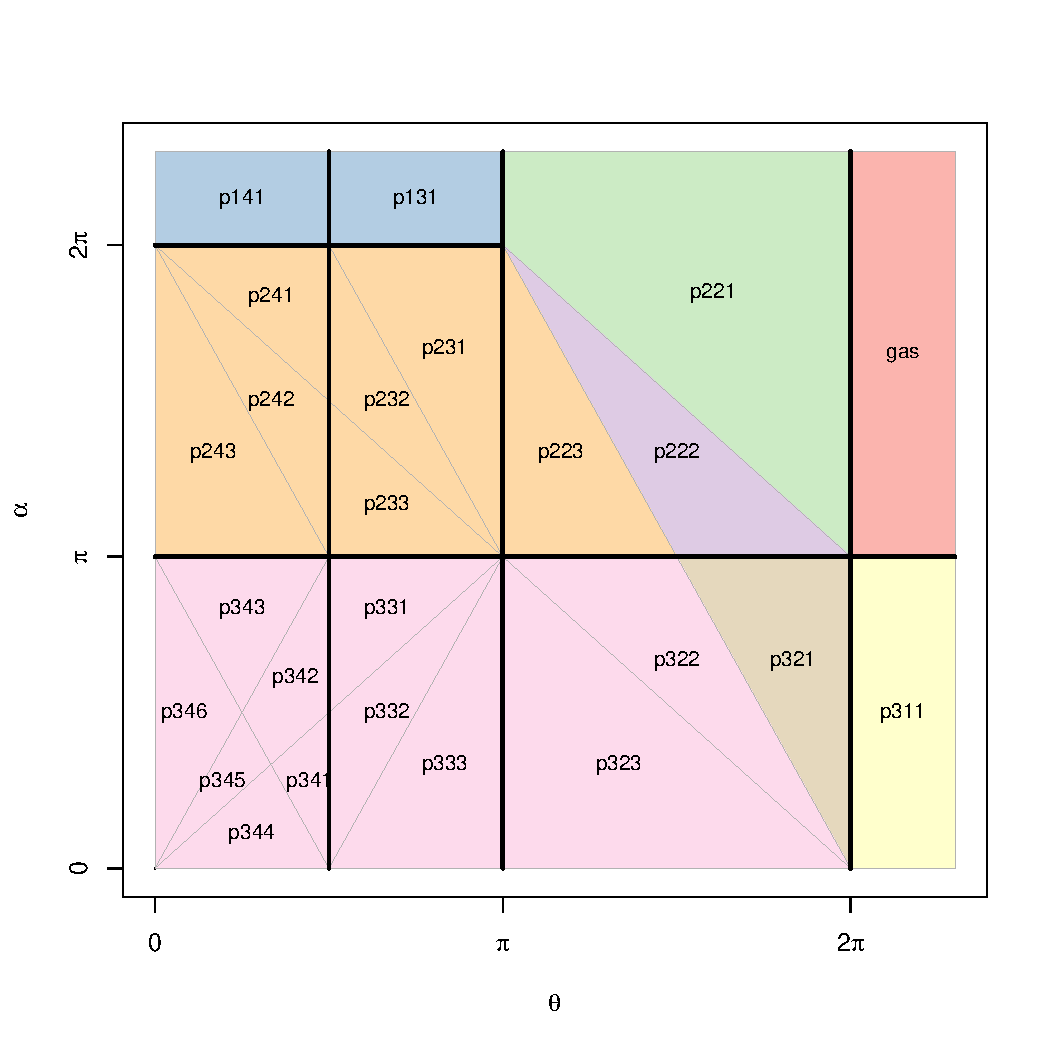
\includegraphics[width=1\textwidth]{imgs/equalRegions.pdf}
\caption{The independently derived models for the whole of parameter space. Regions whose solution for $p$ are equal are coloured similarly. Models are numbered by their row, column and then numbered within that cell (black lines). The models for $\alpha = 2\pi$ or $\theta =  2\pi$ are shown by extending these regions outside of their real boundaries.}
\label{f:regions}
\end{figure}

For regions with profiles that are more complex than a circle we need to explicitly write functions for the width of the profile for every approach angle. We then use these functions to find the average profile for all approach angles by integrating across all $2\pi$ angles of approach and dividing by $2\pi$. In practice, as the models are all left/right symmetrical we can integrate across $\pi$ angles of approach and divide by $\pi$.

\subsubsection{Example derivation}

To work through one example that contains both $\theta$ and $\alpha$ we will examine p321. All other derivations are included in S2. We use $x_i$ to denote the focal angle which is the angle we integrate over. The subscript $i$ distinguishes different angles. For model p321 we examine $x_1$ with  $x_1 = \pi/2$ being an approach angle directly towards the sensor (see Figure~\ref{f:xis}). \cite{rowcliffe2008estimating} use the notation $\gamma_i$ with different numbering.

We can see that, rotating anticlockwise, from $x_1  = \pi/2$ the detection region is $2r$ wide. However, an animal will only be detected if it approaches the detector so that as it enters the detection region the angle between the direction of approach and the direction towards the sensor is less than $\alpha/2$. The width of the profile within which the animal will be detected is therefore $2r\sin(\alpha/2)$. At $x_1  = \theta/2 + \pi/2 - \alpha/2$ we reach a point where the right hand side of the profile (relative to the approach direction) is not limited by the call angle but is limited by the detection angle instead. From here the profile width is therefore $r\sin( \alpha/2) + r\cos( x_1  - \theta/2)$. Finally, at $x_1  = 5\pi/2 - \theta/2  - \alpha/2$ an animal can again be detected from the right side of the detector; the approach angle is far enough round to see past the `blind spot' of the sensor. In this region, until $x_1  = 3\pi/2$, the width of the profile is again $2r\sin( \alpha/2)$. We have therefore characterised the profile width for $\pi$ radians of rotation (from directly towards the sensor to directly behind the sensor.) To find the average profile width for any angle of approach, we integrate these functions over their appropriate intervals of $x_1 $ and divide by $\pi$ giving us:

\begin{align}
    p321 =&\frac{1}{\pi} \left(\int\limits_{\frac{\pi}{2}}^{\frac{\pi}{2} + \frac{\theta}{2} - \frac{\alpha}{2}}2 r \sin{\left (\frac{\alpha}{2} \right )}\;\mathrm{d}x_1+\int\limits_{\frac{\pi}{2} + \frac{\theta}{2} - \frac{\alpha}{2}}^{\frac{5 \pi}{2} - \frac{\theta}{2} - \frac{\alpha}{2}}r \sin{\left (\frac{\alpha}{2} \right )} + r \cos{\left (x_1 - \frac{\theta}{2} \right )}\;\mathrm{d}x_1+\int\limits_{\frac{5 \pi}{2} - \frac{\theta}{2} - \frac{\alpha}{2}}^{\frac{3 \pi}{2}}2 r \sin{\left (\frac{\alpha}{2} \right )}\;\mathrm{d}x_1\right)\\
    p321 =& \frac{r}{\pi} \left(\theta \sin{\left (\frac{\alpha}{2} \right )} - \cos{\left (\frac{\alpha}{2} \right )} + \cos{\left (\frac{\alpha}{2} + \theta \right )}\right) \label{e:p321}
\end{align}

Then, as with the gas model, this term is used to calculate density
\begin{equation}
D = z/vtp321
\end{equation}
We can also see what causes this model to be discontinuously different to p322. Examine the profile at $x_1 = 	\theta/2 + \pi/2$ (the profile is perpendicular to the edge of the blind spot.) We see that there is potentially a case where the left side of the profile is $r\sin( \alpha/2)$ while the right side is zero. This profile doesn't exist if we return to the full $2r\sin( \alpha/2)$ profile before $x_1  = \theta/2 + \pi/2$. Therefore we solve $5\pi/2 - \theta/2 - \alpha/2 <  \theta/2 + \pi/2$. We find that this new profile only exists if $ \alpha < 4\pi - 2 \theta$. This inequality defines the line separating p321 and p322.

While specifying the models had to be done by hand, the calculation of the solutions was done using SymPy \citep{sympy} in Python. 

The models are checked for errors with a number of tests. They are checked against each other by checking that models that are adjacent in parameter space are equal at the boundary between them (e.g. eqn~\ref{e:p321} is equal to 2r as in the gas model when $\alpha=\pi$ and $\theta=2\pi$). Models that border $ \alpha = 0$ should have $p = 0$ when $ \alpha = 0$ and this is checked for (e.g. eqn~\ref{e:p321} is zero when $\alpha=0$ and $\theta=2\pi$). We checked that all solutions are between 0 and $2r$ and that each integral, divided by the range of angles that it is integrated over is between 0 and $2r$. These tests, as well as analytical derivations, are in supplementary script S3.


To make the application of these models simple, we have included an R script in S1. 

\subsection{Simulation Methods}

% @liz: Why is it 56.25km^2? 

The simulated world consists of a  \SI{7.5}{\kilo\meter} by \SI{7.5}{\kilo\meter} square and is populated with a density of  \SI{70}{\animals\per\kilo\meter\squared} \citep{damuth1981population}, creating a total of 3937 animals per simulation randomly placed at the start of the simulation. To reduce computation effort, simulations were run at  \SI{70}{\animals\per\kilo\meter\squared} and then subsampled to achieve lower densities.

The animals move with a simple movement model. The animals moves in discrete time steps but movement is assumed to be continuous. There is no directional change at the end each step. The simulation lasts for $N$ steps of length $T$ during which the animals move with an average constant speed, $v$. 

% @liz. Any reason to wrap stuff in mathnormal? Not sure it's needed. 
% Also the style guide (which I've copied into README.md) says use km^-1 rather than /km so I've put that in.
% Also, not sure it's the best plan but I've switched to units using the siunitx package. This seems the most consistent and will be easiest to change everything consistently if need be.
% changed t to T as t is used above.

The distance travelled in each time step, $\mathnormal{d}$, is a random distance picked from Normal distribution with mean distance, $\mu_d = vT$,  and standard deviation of $\sigma_d = vT/10$. An average speed, $v = $ \SI{40}{\kilo\meter \per \day}, was chosen as this represents the largest day range of terrestrial animals \citep{carbone2005far}, and represents the upper limit of realistic speeds. In order to assess the precision of the analytical models for different sampling conditions and animal behaviours, the results of the movement simulation have been subsampled, and rerun with different movement parameters. The total sampling time that the simulation generates, and density population have been subsampled from the original run. Additional simulations have been run to simulate a range of speeds, between \SI{10}{\meter\per\day} through to \SI{40}{\kilo\meter\per\day} to look at full range of terrestrial movement speeds \citep{carbone2005far}.
  
Additional simulations were also run for more complex movement models, such as, correlated random walks, and stationary, or perching, time steps whilst keeping the same longterm average speed. Further simulations were run to identify the sensitivity of the sensor to changes in the radius and width of the detection angle.

The simulation of movement outputs the details of each individual capture events, including the angle of front of the animal to the sensor, from which the number of capture event can be calculated for different call widths. The total number of capture events are summed and the analytical model applied to the results in order to estimate the density in the simulation. From this the difference between the true, and estimated, densities can be used to evaluate the bias in the analytical models. If the analytical models are correct the mean difference between the two values should converge to zero as sample size increases. 



\section{Results}

\subsection{Analytical results}

Model results have been derived for each region in Figure~\ref{f:regions} with all models except the gas model and p141 being newly derived here. However, many models, although derived seperately, have the same expression for $p$. Figure~\ref{f:equalModelResults} shows the expression for $p$ in each case. The general equation for density, using the correct model for $p$ is then
\begin{equation}
	D = z/pvt.
\end{equation}

Although more thorough checks are performed in S3, it can be seen that all adjacent expressions in Figure~\ref{f:equalModelResults} are equal when expressions for the boundaries between them are substituted in.

\begin{figure}
\centering
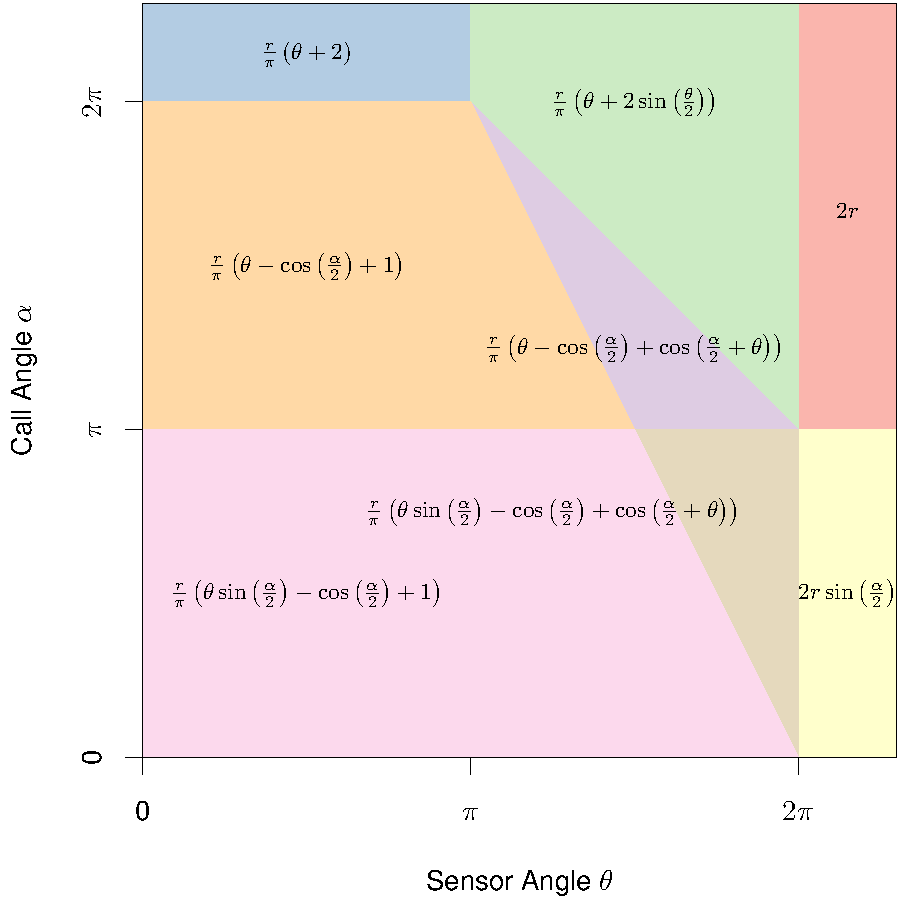
\includegraphics[width=1\textwidth]{imgs/equalModelResults.pdf}
\caption{The results of the models grouped so that all the regions with equal results are presented only once.}
\label{f:equalModelResults}
\end{figure}



\subsection{Simulation results}

A hundred simulations were completed for each of the model derivations, with a density of   \SI{70}{\animals\per\kilo\meter\squared}, for \SI{150}{\day} of simulated time, straight-line movement at a speed of \SI{40}{\kilo\meter\per\day} and a sensor with \SI{100}{\meter} radius. None of the estimated densities produced showed significant deviation from the true density in the simulation, Figure~\ref{f:ModelBias}.
\begin{figure}
\centering
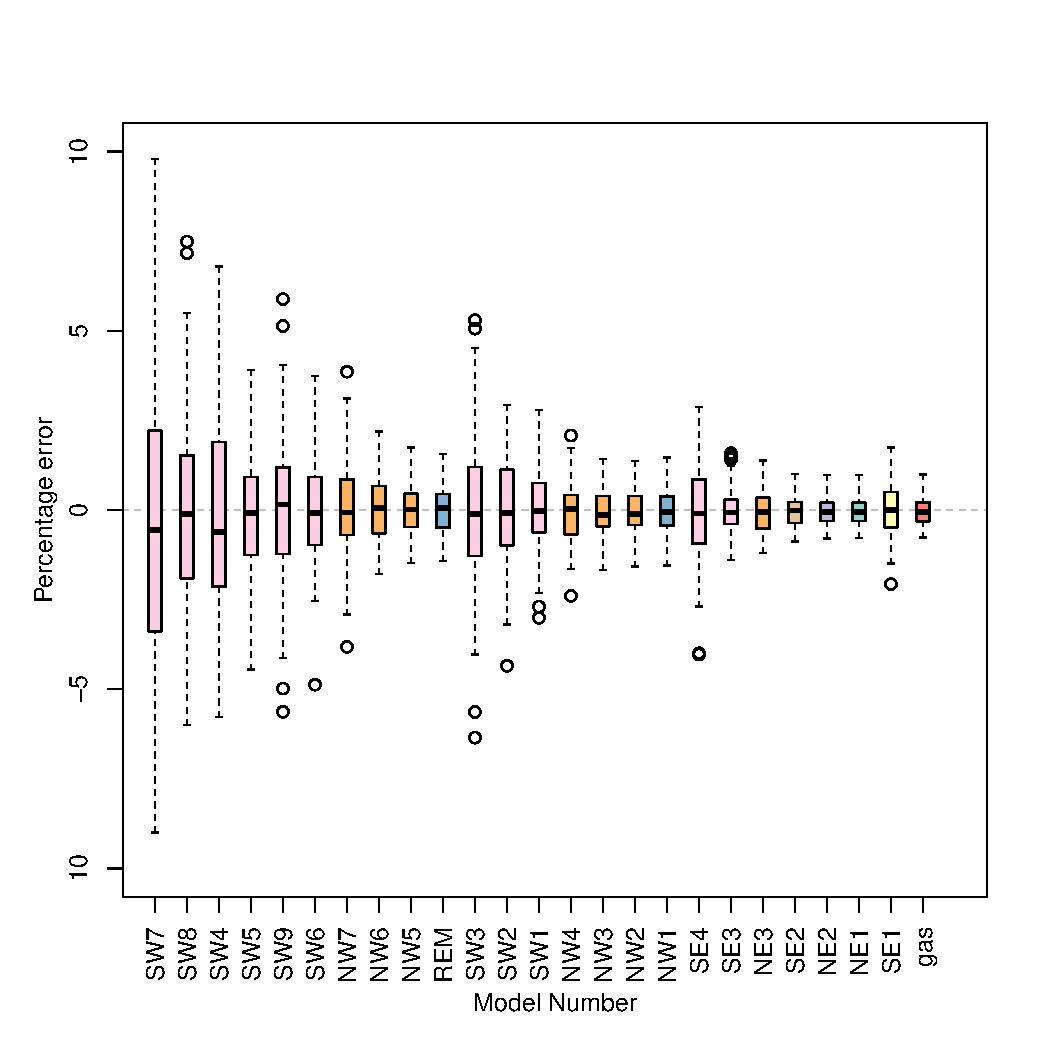
\includegraphics[width=1\textwidth]{imgs/AverageModelBias.pdf}
\caption{The average density estimation bias generated by the simulation per model derivation, shown with 95\% confidence intervals. Simulation settings were: $r = $\SI{100}{\meter}; $t = $\SI{150}{\day}; $v = $ \SI{40}{\kilo\meter\per\day}; $D=$\SI{70}{\animals\per\kilo\meter\squared}; and with angles varying between models.}
\begin{comment} 
p344: $\alpha$= 0.3491; $\theta$=0.2856.  
 p345: $\alpha$= 0.3491; $\theta$=0.5712.
 p346: $\alpha$= 0.3491; $\theta$=0.8568.
 p244: $\alpha$= 0.3491; $\theta$=1.4280.
 p242: $\alpha$= 0.3491; $\theta$=1.7136.
 p241: $\alpha$= 0.3491; $\theta$=2.5704.
 p141: $\alpha$= 0.3491; $\theta$=3.1416.
 p341: $\alpha$= 0.6981; $\theta$=0.2856. 
 p342: $\alpha$= 0.6981; $\theta$=0.8568.
 p333: $\alpha$= 1.0472; $\theta$=0.2856.      
 p332: $\alpha$= 1.0472; $\theta$=0.8568.
 p331: $\alpha$= 1.0472; $\theta$=1.4280.
 p233: $\alpha$= 1.0472; $\theta$=1.7136.
 p232: $\alpha$= 1.0472; $\theta$=2.5704.
 p231: $\alpha$= 1.0472; $\theta$=2.8560.
 p131: $\alpha$= 1.0472; $\theta$=3.1416.
 p323: $\alpha$= 1.7453; $\theta$=0.2856.  
 p322: $\alpha$= 1.7453; $\theta$=1.4280.
 p223: $\alpha$= 1.7453; $\theta$=1.7136.       
 p321: $\alpha$= 2.7925; $\theta$=1.4280.         
 p222: $\alpha$= 2.7925; $\theta$=1.7136. 
 p221: $\alpha$= 2.7925; $\theta$=2.8560.       
 p311: $\alpha$= 3.1416; $\theta$=0.2856.  
 Gas: $\alpha$= 3.1416; $\theta$=2.8560.  
                                     
    }
\end{comment}
\label{f:ModelBias}
\end{figure}

\begin{itemize}
%\item Bias is approximately zero for all models as demonstrated by simulation: 
%	\begin{itemize}
%	\item At a given speed, density, sampling effort, sensor radius, and a given movement strategy
%	\end{itemize}	
\item The expected number of captures will vary, dependent on the system that is being monitored and how it is monitored. This will affect the precision of the estimated: 
	\begin{itemize}
	\item Animal movement strategy
	\item Speed of movement
	\item Density of the animal
	\item Sampling effort
	\item Radius of the sensor
	\end{itemize}
\end{itemize}


\section{Discussion}

%• Discussion: Point out the importance of the results and place them in the context of previous studies and in relation to the application of the work (expanding on the Synthesis and applications section of the Summary). Where appropriate, set out recommendations for management or policy.

We have developed a number of models that can be used to estimate density from acoustic and optical sensors. This has entailed a generalisation of the gas model and the model in \cite{rowcliffe2008estimating} to be applicable to any combination of sensor width and call directionality. 

We have used simulations to show, as a proof of principle, that these models are accurate and precise. We have broken  the ideal gas assumptions of animal movement and still retained accurate results, although precision is lowered. Finally we have given some general advise on best practice, although this is given based on similar assumptions those used in the derivation in the models.

These model are therefore available to for the estimation of density of a number of taxa of importance to conservation, zoonotic diseases and ecosystem services. The models are suitable for certain groups for which there are currently no, or few, effective methods for density estimation. 

Importantly the methods are noninvasive and do not require human marking (as required for mark recapture models). This makes them suitable for large, continuous monitoring projects with limited human resources. It also makes them suitable for sensitive species or species that are difficult or dangerous to catch.

Although we have used simulations to validate these models, much more robust testing is needed. Although difficult, proper field test validation would be required before the models could be fully trusted. Note, however, that the gas model and model of \cite{rowcliffe2008estimating} have been been field tested and many of the assumptions between these models and those derived here are the same. As the utility of the models is that they can be used with taxa that are difficult to study with other methods, there are not many obvious groups that have reliable, gold standard estimates of density from other methods that could then be used to validate these models.

As easier way to continue to evaluate the models is to run more extensive simulations which break the assumptions of the analytical models. The main element that cannot be analytically treated is the complex movement of real animals. Therefore testing these methods against true animal traces, or more complex movement models would be useful.

There are many possible extensions to these models. As has been noted before \citep{rowcliffe2008estimating,Hutchinson_Waser_2007} altering the equations to estimate animal density of group living species is relatively simple. However, the models herein would have to be carefully rederived to account for group living as directional calls are not considered in previous work, and may have important effects.

The original gas model was formulated for the case where both the animal population and the sensors are moving. Indeed any of the models with animals that are equally detectable in all directiosn ($\alpha = 2\pi$) can be trivially expanded for moving by substituting the sum of the average animal velocity and the sensor velocity for $v$ as used here. However, when the animal has a directional call, the extension becomes much less simple. The approach would be to calculate again the mean profile width. However, for each angle of approach, one would have to average the profile width for an animal facing in any direction (i.e. not necessarily moving towards the sensor) weighted by the relative velocity of that direction.

An interesting, and so far untackled problem, is edge effects caused by trigger delays (the delay between sensing an animal and attempting to record the encounter) and time expansion acoustic detectors which repeatedly turn on an off during sampling. Both of these have potential biases as animals can move through the detection region without being detected. The models herein are formulated assuming constant surveillance and so the error quickly becomes negligable.




\begin{comment}

\begin{itemize}
\item Developed a number of models that can be used to estimate density from acoustic and optical sensors 
\item These models are accurate 
\item Implications for best practice:
	\begin{itemize}
	\item Densities of above X converge quickly to a stable mean
	\item Animals which have an average speed of greater then X 
	\item Surveys of at Xhrs of effort produce stable results
	\end{itemize}
\item Aspirational stuff for the future:
	\begin{itemize}
	\item Consider animals moving in groups
	\item Incorporating more realistic movement strategies
	\item Moving detectors
	\item Trigger delays and time expansion
	\end{itemize}
\end{itemize}

\end{comment}


%\section{Acknowledgements}



%\section{Data Accessibility}




\begin{table}[t]
\centering
\begin{tabular}{lll}
Symbol 	& Description & Units\\\hline
$v$		& Velocity & \SI{}{\meter\per\second}\\
$\theta$	& Angle of detection & Radians \\
$\alpha$	& Animal call/beam width & Radians \\
$r$ 		& Detection distance & Metres\\
$p$ 		& Average profile width & Metres\\
$t$		& Time & Seconds\\
$z$		& Number of dections & \\
$D$		& Animal density & \SI{}{\animals\per\meter\squared} \\
$x_i$	        & Focal Angle $i \in \{1,2,3,4\} $ 	& Radians\\
$T$ 		& Step length & Seconds\\
$N$ 		& Number of steps per simulation & \\
$d$ 		& Time step index &

\end{tabular}
\caption{List of symbols used}
\label{t:paras}
\end{table}



\bibliographystyle{mee.bst}	
\bibliography{lucas-moorcroft-etal-refs.bib}	


\end{document}
		
